\begin{figure}[h!]
    \centering
    \caption{Effects of \emph{Plan Cuadrante} by Resource Increase: Trust, Complaints, and Arrests}
    \label{fig:heterogeneity_appendix}
    \begin{subfigure}[t]{0.48\textwidth}
        \centering
        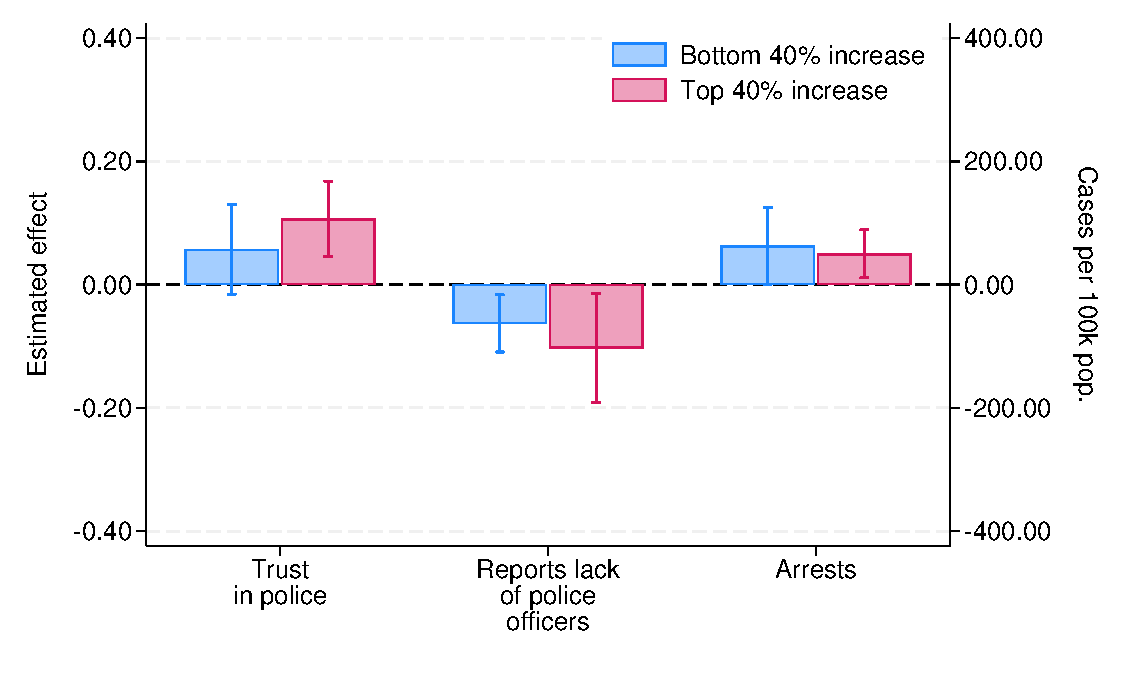
\includegraphics[width=\linewidth]{../manuscript/Graphs/heterogeneity_off_appendix.pdf}
        \caption{By the intensity of $\Delta$ in police officers}
    \end{subfigure}\hfill
    \begin{subfigure}[t]{0.48\textwidth}
        \centering
        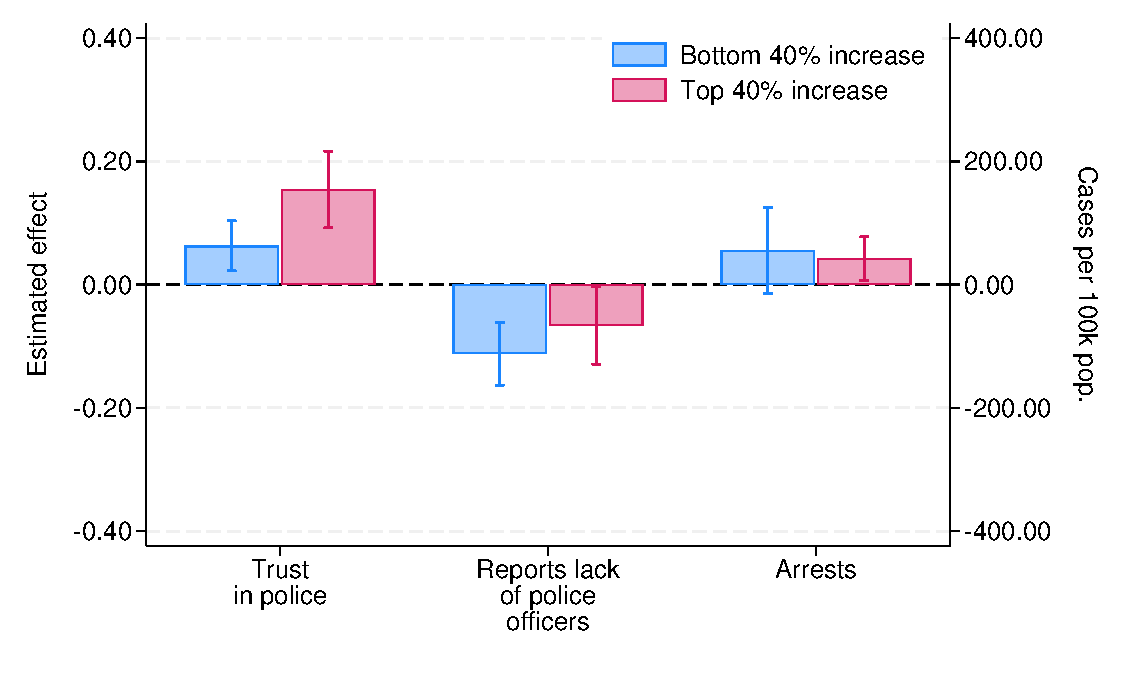
\includegraphics[width=\linewidth]{../manuscript/Graphs/heterogeneity_pv_appendix.pdf}
        \caption{By the intensity of $\Delta$ in patrol vehicles}
    \end{subfigure}
    \\[8pt]
    \begin{minipage}{0.99\textwidth}
    \footnotesize Notes: This figure complements Figure \ref{fig:figure_resources} by reporting, for the three outcomes not shown there, the effect of \emph{Plan Cuadrante} estimated separately for municipalities in the bottom 40\% (blue) and top 40\% (red) of the resource-increase distribution. Panel (a) splits municipalities by the increase in police officers and panel (b) by the increase in patrol vehicles. In each panel, arrests (administrative data, in cases per 100,000 inhabitants) are read on the right axis; the other two outcomes, from the ENUSC survey (trust in the police, and reports about the lack of police officers), are read on the left axis. Effects are estimated using the difference-in-differences estimator for staggered treatment adoption developed in \citet{Callaway}; bars are point estimates and whiskers 95\% confidence intervals, with standard errors clustered at the municipality level using the wild bootstrapping procedure.
    \end{minipage}
\end{figure}
